\documentclass[12pt, a4paper]{article}

% ── Encoding & Language ───────────────────────────────────────────────────────
\usepackage[utf8]{inputenc}
\usepackage[T1]{fontenc}
\usepackage[ngerman]{babel}

% ── Layout ───────────────────────────────────────────────────────────────────
\usepackage[top=2.5cm, bottom=2.5cm, left=3cm, right=2.5cm]{geometry}
\usepackage{setspace}
\onehalfspacing
\setlength{\parindent}{0pt}
\setlength{\parskip}{6pt}

% ── Fonts ────────────────────────────────────────────────────────────────────
\usepackage{lmodern}

% ── Math ─────────────────────────────────────────────────────────────────────
\usepackage{amsmath, amssymb}

% ── Tables ───────────────────────────────────────────────────────────────────
\usepackage{booktabs}
\usepackage{tabularx}
\usepackage{longtable}
\usepackage{multirow}
\usepackage{array}
\usepackage{float}

% ── Graphics ─────────────────────────────────────────────────────────────────
\usepackage{graphicx}
\usepackage[labelfont=bf, skip=6pt]{caption}
\usepackage{subcaption}
\graphicspath{{figures/}{figures/02_sentiment_analysis/}{figures/03_correlation_modeling/}}

% ── Colors ───────────────────────────────────────────────────────────────────
\usepackage[dvipsnames]{xcolor}
\definecolor{linkblue}{HTML}{1A5276}

% ── Hyperlinks ───────────────────────────────────────────────────────────────
\usepackage[
  colorlinks=true,
  linkcolor=linkblue,
  citecolor=linkblue,
  urlcolor=linkblue,
  pdfauthor={Ilker},
  pdftitle={Web Mining: Sentiment-Analyse von X (Twitter) und Aktienkursrenditen},
]{hyperref}
\usepackage{url}

% ── Code listings ────────────────────────────────────────────────────────────
\usepackage{listings}
\lstset{
  basicstyle=\ttfamily\small,
  breaklines=true,
  frame=single,
  backgroundcolor=\color{gray!8},
  keywordstyle=\color{blue},
  commentstyle=\color{gray},
  stringstyle=\color{orange!80!black},
}

% ── Bibliography ─────────────────────────────────────────────────────────────
\usepackage[
  backend=biber,
  style=authoryear,
  sorting=nyt,
  maxnames=3,
]{biblatex}
\addbibresource{references.bib}

% ── Misc ─────────────────────────────────────────────────────────────────────
\usepackage{enumitem}
\usepackage{microtype}
\usepackage{csquotes}

% ─────────────────────────────────────────────────────────────────────────────

\begin{document}

% ── Title Page ───────────────────────────────────────────────────────────────
\begin{titlepage}
  \centering
  \vspace*{2cm}

  {\LARGE\bfseries Web Mining: Sentiment-Analyse von X\,(Twitter)\\
  und Aktienkursrenditen\par}

  \vspace{1.5cm}
  {\large Modularbeit im Rahmen des Moduls \textit{Web Mining}\\
  M.\,Sc. Data Science\par}

  \vspace{2cm}
  {\large Ilker\par}

  \vspace{0.5cm}
  {\normalsize Hochschule\par}

  \vfill
  {\normalsize \today\par}
\end{titlepage}

% ── Table of Contents ────────────────────────────────────────────────────────
\tableofcontents
\newpage

% ── Sections ─────────────────────────────────────────────────────────────────
\section{Einleitung}
\label{sec:einleitung}

Soziale Medien haben sich in den vergangenen Jahren zu einer bedeutenden Informationsquelle für Finanzmärkte entwickelt. Plattformen wie X\,(ehem.\ Twitter) ermöglichen es, öffentlich zugängliche Stimmungsäußerungen von Marktteilnehmern in nahezu Echtzeit zu beobachten. Gleichzeitig sind Aktienkurse von Informationen und kollektiven Erwartungen abhängig, die sich über digitale Kanäle rasch verbreiten. Diese Arbeit untersucht daher die Frage, ob und in welchem Ausmaß das auf X\,(Twitter) gemessene Sentiment von Marktteilnehmern mit den Kursrenditen ausgewählter Unternehmen zusammenhängt.

\subsection*{Forschungsfrage}

Die zentrale Forschungsfrage lautet:

\begin{quote}
\textit{Lässt sich aus dem täglichen Sentiment auf X\,(Twitter) ein statistisch signifikanter Zusammenhang mit den Tagesrenditen börsennotierter Unternehmen aus den Bereichen Energie, Elektromobilität und Wärmepumpen ableiten?}
\end{quote}

Konkret wird untersucht, ob Sentiment-Signale den Kursrenditen vorausgehen, ihnen folgen oder ob kein erklärender Zusammenhang besteht. Dabei wird auch geprüft, ob vergangenes Sentiment im Sinne des Granger-Kausalitätstests Vorhersageinformation über zukünftige Renditen enthält.

\subsection*{Fokus und Relevanz}

Das Untersuchungsfeld umfasst zwölf Unternehmen aus drei thematischen Segmenten: etablierte Energiekonzerne (BP, ExxonMobil, Shell, TotalEnergies, Eni), Hersteller von Wärmepumpen und Klimatisierungstechnik (Daikin, NIBE, Carrier Global, Mitsubishi Electric) sowie Automobilhersteller mit Elektromobilitätsfokus (Tesla, BYD, Volkswagen, Hyundai). Diese Auswahl ist relevant, weil sie Unternehmen umfasst, die von laufenden Diskursen über Energiewende und Klimapolitik betroffen sind und daher eine erhöhte Exposition gegenüber öffentlichem Sentiment erwarten lassen.

\subsection*{Beitrag und Aufbau}

Der Beitrag dieser Arbeit liegt in der Verknüpfung eines aktuellen, selbst erhobenen Social-Media-Datensatzes mit historischen Börsenkursdaten sowie in der systematischen Anwendung mehrerer quantitativer Methoden auf diesen spezifischen Ausschnitt. Abschnitt~\ref{sec:methodik} beschreibt die Datenerhebung, Datenaufbereitung und die eingesetzten Analysemethoden. Abschnitt~\ref{sec:ergebnisse} stellt die Ergebnisse dar. Abschnitt~\ref{sec:diskussion} bewertet diese kritisch, geht auf Limitationen ein und ordnet die Befunde in den Forschungskontext ein. Abschnitt~\ref{sec:fazit} schließt mit einem Fazit.

\newpage

\section{Methodik}
\label{sec:methodik}

Die Analyse gliedert sich in drei aufeinander aufbauende Schritte: Datenerhebung und Qualitätsprüfung, Sentiment-Analyse sowie Korrelationsmodellierung. Jeder Schritt entspricht einem Jupyter-Notebook (\texttt{01\_data\_quality\_eda.ipynb}, \texttt{02\_sentiment\_analysis.ipynb}, \texttt{03\_correlation\_modeling.ipynb}).

% ─────────────────────────────────────────────────────────────────────────────
\subsection{Datenerhebung und explorative Qualitätsprüfung}
\label{subsec:eda}

\subsubsection*{Vorgehen}

Im ersten Schritt wurde die strukturelle Qualität der erhobenen Daten geprüft.
Grundlage bildeten die in einer SQLite-Datenbank gespeicherten Tweets, Tweet-Snapshots und Intraday-Preissnapshots sowie separat vorliegende historische Tagespreise, die über die Bibliothek \textit{yfinance} bezogen und in einer CSV-Datei abgelegt wurden. Ziel dieses Schritts war es, Datenlücken, Abdeckungsunterschiede zwischen Unternehmen und potenzielle Verzerrungen sichtbar zu machen, bevor inhaltliche Sentiment-Scores berechnet wurden. Dazu wurden Zeitstempel vereinheitlicht, ein Startzeitraum ab dem 01.\,01.\,2026 angewendet und die Analyse auf die in einer Konfigurationsdatei definierten Fokus-Ticker beschränkt.

Für die inhaltliche Zuordnung der Tweets zu den Fokus-Unternehmen wurde ein zweistufiges Matching-Verfahren verwendet. Im ersten Schritt wurden vorhandene Cashtags bzw. Symbolspalten direkt bekannten Ticker-Aliasen zugeordnet. Im zweiten Schritt wurden Tweets ohne Symbolangabe anhand regulärer Ausdrücke auf Unternehmensnamen, Cashtags und markenspezifische Begriffe geprüft. Dadurch konnten auch Beiträge erfasst werden, die nicht explizit mit einem Börsenkürzel versehen waren. Ergänzend wurden Tweets mit und ohne substanziellen Inhalt unterschieden: URLs, Mentions und Cashtags wurden entfernt und nur Beiträge mit mindestens 20~verbleibenden Zeichen als inhaltlich aussagekräftig markiert.

Ein weiterer methodischer Bestandteil war die Identifikation strukturell auffälliger Tweets. Dazu wurden Retweets über das Präfix \enquote{RT @} markiert sowie Kandidaten für nicht-organische Aktivität geprüft. Engagement-Snapshots wurden zusammengeführt, um erste Aussagen über Reichweite und Interaktionsdynamik zu ermöglichen. Viral aktive Tweets wurden über das 95.\,Perzentil der Engagement-Velocity (Likes pro Minute zwischen erstem und letztem Snapshot) identifiziert.

\subsubsection*{Datensätze}

Verwendet wurden die Tabellen \texttt{tweets}, \texttt{tweet\_snapshots} und \texttt{price\_snapshots} aus der SQLite-Datenbank sowie die historischen Tagespreise aus \texttt{prices.csv}. Die Tweets enthalten Autor, Inhalt, Posting-Zeitpunkt und teils ein extrahiertes Symbol. Die Snapshots liefern Engagement-Metriken (Likes, Retweets) und kursbezogene Momentaufnahmen.

\subsubsection*{Beobachtungen}

Die Analyse ergab, dass die Ticker-Zuweisung initial für mehrere Unternehmen zu geringe Abdeckungen lieferte. Als Ursache wurden zu eng gefasste Wortgrenzen in den regulären Ausdrücken identifiziert: Ausdrücke der Form \texttt{\textbackslash bWORD\textbackslash b} konnten zusammengesetzte Hashtags wie \textit{\#TeslaStock} oder \textit{\#NIBEHeatPump} nicht erfassen, da der Wortgrenzenoperator einen Folgebuchstaben nicht zulässt. Die Muster wurden daraufhin angepasst. Tabelle~\ref{tab:coverage} zeigt die resultierende Abdeckung je Ticker.

\begin{table}[H]
\centering
\caption{Abdeckung der Fokus-Ticker im bereinigten Datensatz (Zeitraum ab 01.01.2026)}
\label{tab:coverage}
\begin{tabular}{lrr}
\toprule
\textbf{Ticker} & \textbf{Tweet-Tage} & \textbf{Sentiment-Tage} \\
\midrule
TSLA   & 124 & 68 \\
VWAGY  &  91 & 53 \\
XOM    &  72 & 41 \\
BYDDY  &  59 & 34 \\
BP     &  50 & 27 \\
TTE    &  38 & 23 \\
6503.T &  29 & 17 \\
6367.T &  17 & 11 \\
E      &   9 &  7 \\
SHEL   &   8 &  5 \\
CARR   &   9 &  3 \\
NIBE-B.ST &  2 &  1 \\
\bottomrule
\end{tabular}
\end{table}

% ─────────────────────────────────────────────────────────────────────────────
\subsection{Sentiment-Analyse}
\label{subsec:sentiment}

\subsubsection*{Modellauswahl}

Für die Sentiment-Klassifikation wurde \texttt{cardiffnlp/twitter-xlm-roberta-base-sentiment} als Primärmodell eingesetzt \autocite{loureiro2022timelms}. Die Wahl dieses Modells war methodisch sinnvoll, weil der Datensatz nicht nur englische, sondern auch deutsch-, französisch- und japanischsprachige Tweets enthält. Das Modell basiert auf XLM-RoBERTa \autocite{conneau2020unsupervised} und ist speziell auf Twitter-Daten trainiert. Es klassifiziert jeden Eingabetext in eine von drei Klassen: \textit{Positive}, \textit{Neutral}, \textit{Negative}. Zusätzlich stellt es Klassenwahrscheinlichkeiten bereit, aus denen ein kontinuierlicher Compound-Score gebildet wurde:

\begin{equation}
\text{xlm\_compound} = P(\text{positive}) - P(\text{negative}) \in [-1,\, 1]
\label{eq:compound}
\end{equation}

Als Baseline wurde ergänzend VADER (Valence Aware Dictionary and sEntiment Reasoner) eingesetzt \autocite{hutto2014vader}. Da VADER auf einem englischen Lexikon basiert, ist es für nicht-englische Tweets nicht valide. Es diente daher ausschließlich als Vergleichsmaßstab für den englischsprachigen Anteil des Datensatzes.

\subsubsection*{Datenfilterung}

Vor der Modellinferenz wurden zwei Filtermaßnahmen angewendet:

\begin{enumerate}[noitemsep]
\item \textbf{Bot-Filterung:} Als Bot-Kandidat wurde jeder Account definiert, der keine Follower besitzt und zugleich mindestens drei Tweets im Datensatz veröffentlicht hat. Diese Regel ist als konservativer Proxy für nicht-organische Aktivität zu verstehen.
\item \textbf{Content-Filter:} Die Inferenz wurde ausschließlich auf Tweets angewendet, die nach Entfernung von URLs, Mentions und Cashtags noch mindestens 20~Zeichen enthielten.
\end{enumerate}

Die Sprache jedes Tweets wurde außerdem mit \textit{langdetect} automatisch erkannt, um die Übereinstimmung zwischen XLM-RoBERTa- und VADER-Ergebnissen sprachspezifisch auswerten zu können.

\subsubsection*{Retweet-Separation}

Original-Tweets und Retweets wurden getrennt verarbeitet, um zu vermeiden, dass die bloße Weiterverbreitung von Inhalten das Sentiment-Signal verzerrt. Als Retweet wurde jeder Beitrag eingestuft, der mit dem Präfix \enquote{RT @} beginnt. Im vorliegenden Datensatz enthielten alle gecrawlten Tweets originären Inhalt; die Trennung war daher analytisch irrelevant, methodisch aber korrekt implementiert.

\subsubsection*{Tägliche Aggregation}

Auf Tweet-Ebene erzeugte Sentiment-Scores wurden je Fokus-Ticker und Kalendertag aggregiert. Die täglichen Aggregate umfassen:

\begin{itemize}[noitemsep]
\item \texttt{mean\_xlm\_compound}: ungewichteter Mittelwert des Compound-Scores
\item \texttt{pct\_positive}, \texttt{pct\_negative}: Anteile positiver und negativer Tweets
\item \texttt{mean\_vader\_en}: mittlerer VADER-Score (nur englische Tweets)
\item \texttt{weighted\_xlm\_compound}: follower-gewichteter Compound-Score als Reichweiten-Proxy
\end{itemize}

Der follower-gewichtete Score gewichtet den Compound-Wert jedes Tweets proportional zu den Follower-Zahlen des Autors:

\begin{equation}
\text{weighted\_xlm} = \frac{\sum_{i} f_i \cdot c_i}{\sum_{i} f_i}
\label{eq:weighted_compound}
\end{equation}

wobei $f_i$ die Follower-Zahl und $c_i$ den Compound-Score von Tweet $i$ bezeichnen. Dieses Signal dient als primäres Sentiment-Maß in der Korrelationsanalyse, da es die Reichweite einzelner Beiträge berücksichtigt.

Abbildung~\ref{fig:follower_weighting} zeigt den Vergleich von ungewichtetem und follower-gewichtetem Compound-Score je Ticker. Die meisten Ticker liegen nahe der Diagonalen, was auf geringe Gewichtungseffekte hindeutet.

\begin{figure}[H]
  \centering
  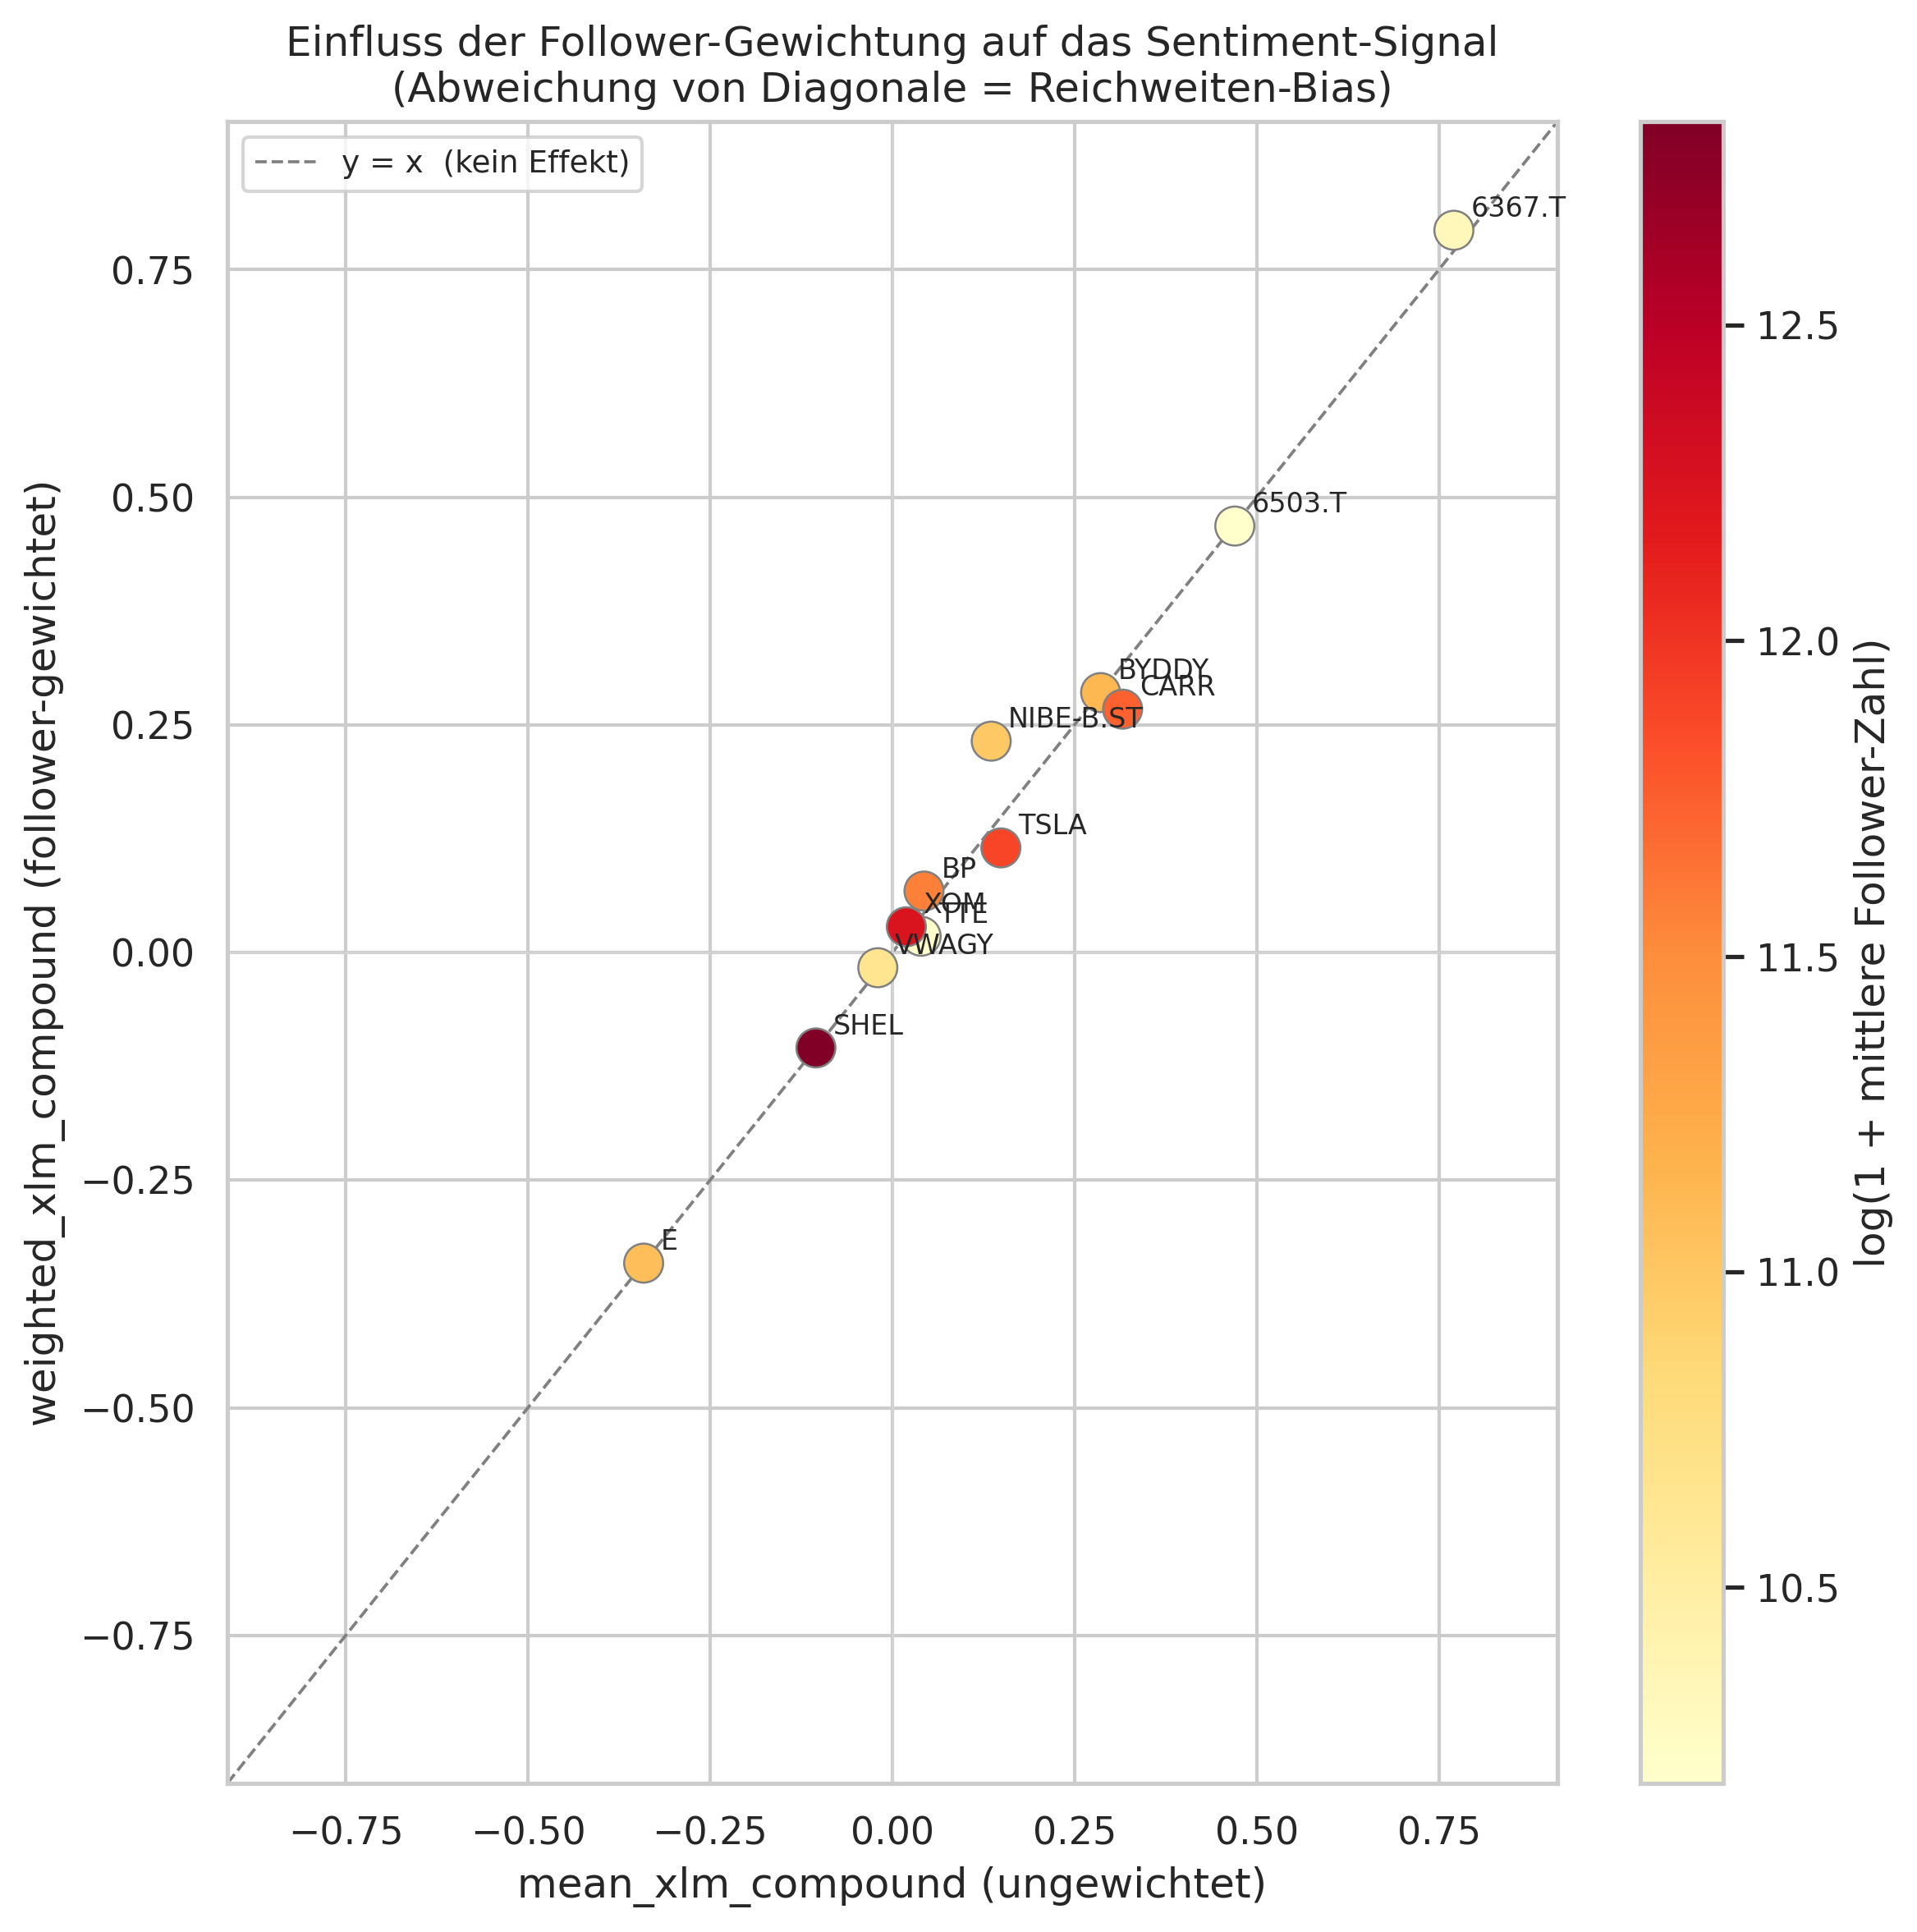
\includegraphics[width=0.72\textwidth]{figures/02_sentiment_analysis/04_follower_weighting_scatter.png}
  \caption{Ungewichteter vs.\ follower-gewichteter mittlerer Compound-Score je Fokus-Ticker. Punkte auf der Diagonalen zeigen keinen Reichweiten-Bias; Einfärbung nach $\log(1 + \text{mittlere Follower-Zahl})$.}
  \label{fig:follower_weighting}
\end{figure}

\subsubsection*{Datensätze}

Als Input dienten die Tweets aus der SQLite-Datenbank. Als Output wurden folgende Parquet-Dateien erzeugt:

\begin{itemize}[noitemsep]
\item \texttt{tweets\_with\_sentiment\_original.parquet} (2\,266 Zeilen, tweet-level)
\item \texttt{daily\_sentiment\_original.parquet} (508 Zeilen, Primärinput für NB03)
\end{itemize}

% ─────────────────────────────────────────────────────────────────────────────
\subsection{Korrelationsmodellierung}
\label{subsec:korrelation}

\subsubsection*{Daten und Zusammenführung}

Als Primärinput für die Korrelationsanalyse wurde \texttt{daily\_sentiment\_original.parquet} verwendet. Retweets wurden bewusst aus der Hauptanalyse ausgeschlossen. Als zentrales Sentiment-Signal diente der follower-gewichtete Compound-Score \texttt{weighted\_xlm\_compound} gemäß Gleichung~\eqref{eq:weighted_compound}.

Die Tagesrendite wurde aus historischen Tagespreisen über einfache prozentuale Veränderung des adjustierten Schlusskurses berechnet:

\begin{equation}
r_t = \frac{P_t - P_{t-1}}{P_{t-1}}
\label{eq:return}
\end{equation}

Die Zusammenführung erfolgte über einen Inner-Join auf Ticker und Datum, sodass nur Tage mit sowohl validem Sentiment-Score als auch gültigem Renditewert in die Analyse eingingen.

\subsubsection*{Overlap-Report und Methoden-Eligibility}

Statt einer globalen Mindeststichprobenschwelle, die Ticker still ausschließt, wurde ein Overlap-Report erstellt. Dieser dokumentiert für jeden Fokus-Ticker die Anzahl der Sentiment-Tage, Preis-Tage und tatsächlich überlappenden Tage sowie methodenspezifische Eligibility-Flags:

\begin{itemize}[noitemsep]
\item \textbf{Pearson/Spearman:} mindestens 5 gepaarte Beobachtungen pro Lag
\item \textbf{Rolling-Korrelation:} mindestens 30 Überlappungstage
\item \textbf{Granger-Test:} mindestens 30 Beobachtungen
\item \textbf{Event-Study:} mindestens 20 Basistage und mindestens 5 Ereignisse je Richtung
\end{itemize}

Dieses Vorgehen stellt sicher, dass alle Ticker im Analysebericht sichtbar bleiben, während gleichzeitig statistisch zu dünne Teilanalysen transparent als nicht belastbar gekennzeichnet werden.

\subsubsection*{Methode 1: Lag-Korrelation (Pearson und Spearman)}

Für Lags $l \in \{0, 1, 2, 3\}$ wurde berechnet, ob der Sentiment-Score am Tag $t$ mit der Rendite am Tag $t+l$ korreliert. Lag~0 entspricht einem gleichzeitigen Zusammenhang, Lags~1--3 einem potenziellen Vorlauf des Sentiments gegenüber der Rendite:

\begin{equation}
r_{\text{Pearson}}(l) = \text{corr}\!\left(\text{sentiment}_t,\; r_{t+l}\right)
\label{eq:pearson_lag}
\end{equation}

Neben dem linearen Pearson-Koeffizienten wurde auch der rangbasierte Spearman-Koeffizient berechnet, um Robustheit gegenüber Ausreißern zu prüfen.

Da für bis zu zehn Ticker bei je vier Lags potenziell 40 Tests durchgeführt werden, wurden alle $p$-Werte mit der Benjamini-Hochberg-Methode (False Discovery Rate, FDR) korrigiert \autocite{benjamini1995controlling}. Berichtete Signifikanz bezieht sich stets auf den adjustierten Wert $p_{\mathrm{adj}}$. Ergänzend wurden 95\,\%-Konfidenzintervalle für den Pearson-Koeffizienten über die Fisher-z-Transformation berechnet:

\begin{equation}
z = \operatorname{arctanh}(r), \quad
\mathrm{SE}_z = \frac{1}{\sqrt{n-3}}, \quad
\mathrm{KI}_{95\%} = \bigl[\tanh(z - 1{,}96 \cdot \mathrm{SE}_z),\; \tanh(z + 1{,}96 \cdot \mathrm{SE}_z)\bigr]
\label{eq:fisher_ci}
\end{equation}

\subsubsection*{Methode 2: Rolling-Korrelation}

Für Ticker mit mindestens 30 überlappenden Tagen wurde ein gleitender Pearson-Korrelationskoeffizient mit einem Fenster von 30 Handelstagen berechnet. Dieser dient dazu, zeitliche Instabilität oder Phasenwechsel im Zusammenhang sichtbar zu machen, die bei aggregierten Gesamtmaßzahlen verborgen bleiben würden.

\subsubsection*{Methode 3: Granger-Kausalitätstest}

Der Granger-Test \autocite{granger1969investigating} prüft, ob vergangenes Sentiment einen zusätzlichen Beitrag zur Vorhersage zukünftiger Renditen leistet -- über die Autokorrelation der Renditen hinaus. Technisch wird ein VAR(l)-Modell geschätzt und über einen F-Test getestet, ob die Sentiment-Lags in der Renditegleichung statistisch signifikant sind. Zur Überprüfung der Stationaritätsvoraussetzung wurden die Sentiment- und Renditereihen jedes für den Granger-Test in Frage kommenden Tickers vorab mit dem Augmented-Dickey-Fuller-Test (ADF) auf Einheitswurzeln geprüft \autocite{dickey1979distribution}. Getestet wurden Lags 1 bis 3. Zu beachten ist, dass Granger-Kausalität keine echte Kausalität im wissenschaftlichen Sinne belegt, sondern lediglich Vorhersageverbesserung anzeigt \autocite{granger1969investigating}.

\subsubsection*{Methode 4: Event-Study}

In der Event-Study wurden Tage identifiziert, an denen der Sentiment-Score um mehr als eine Standardabweichung vom Ticker-Mittelwert abwich:

\begin{equation}
\text{Ereignis}^+ : \; s_t > \bar{s} + \sigma_s, \qquad
\text{Ereignis}^- : \; s_t < \bar{s} - \sigma_s
\label{eq:event_condition}
\end{equation}

Als abnormale Rendite wurde die Differenz zwischen der tatsächlichen Rendite und der Tagesrendite des S\&P\,500-Index (\texttt{\textasciicircum GSPC}) als externem Marktbenchmark definiert. Die S\&P\,500-Daten wurden über \textit{yfinance} bezogen. Diese Wahl vermeidet den methodischen Fehler, den Benchmark aus den Focus-Tickern selbst zu berechnen, was zu einem zirkulären Vergleich geführt hätte. Über alle Ereignisse wurde ein Durchschnitts-CAR-Profil (Cumulated Abnormal Return) im Fenster $t \in [-5, +5]$ Handelstagen berechnet.

\newpage

\section{Ergebnisse}
\label{sec:ergebnisse}

\subsection{Abdeckung und Overlap}
\label{subsec:ergebnisse_abdeckung}

Der Datensatz umfasst nach Bereinigung, Bot-Filterung und Beschränkung auf den Zeitraum ab dem 01.\,01.\,2026 insgesamt 2\,266 Tweets von 12 Fokus-Tickern. Nach Zusammenführung mit den historischen Tagespreisen ergaben sich 290 tatsächlich nutzbare, gepaarte Beobachtungen. Der überlappende Zeitraum erstreckte sich vom 02.\,01.\,2026 bis zum 23.\,04.\,2026.

Tabelle~\ref{tab:overlap} zeigt die Abdeckung je Ticker sowie die Eignung für die vier Analysemethoden. TSLA, VWAGY, XOM und BYDDY erfüllten alle Mindestanforderungen. BP und TTE hatten ausreichend Beobachtungen für Pearson/Spearman und die Event-Study, nicht aber für Rolling-Korrelation und Granger-Test. Für die übrigen Ticker konnten nur vereinzelte Korrelationskoeffizienten berechnet werden.

\begin{table}[H]
\centering
\caption{Overlap-Report: Abdeckung und Methoden-Eligibility je Fokus-Ticker}
\label{tab:overlap}
\begin{tabular}{lrcccc}
\toprule
\textbf{Ticker} & \textbf{Aligned Days} & \textbf{Corr} & \textbf{Rolling} & \textbf{Granger} & \textbf{Event} \\
\midrule
TSLA      & 68 & \checkmark & \checkmark & \checkmark & \checkmark \\
VWAGY     & 53 & \checkmark & \checkmark & \checkmark & \checkmark \\
XOM       & 41 & \checkmark & \checkmark & \checkmark & \checkmark \\
BYDDY     & 34 & \checkmark & \checkmark & \checkmark & \checkmark \\
BP        & 27 & \checkmark & --         & --         & \checkmark \\
TTE       & 23 & \checkmark & --         & --         & \checkmark \\
6503.T    & 17 & \checkmark & --         & --         & --         \\
6367.T    & 11 & \checkmark & --         & --         & --         \\
E         &  7 & \checkmark & --         & --         & --         \\
SHEL      &  5 & \checkmark & --         & --         & --         \\
CARR      &  3 & --         & --         & --         & --         \\
NIBE-B.ST &  1 & --         & --         & --         & --         \\
\bottomrule
\multicolumn{6}{l}{\footnotesize \checkmark = Methode anwendbar; -- = Mindestanforderung nicht erfüllt}
\end{tabular}
\end{table}

% ─────────────────────────────────────────────────────────────────────────────
\subsection{Sentiment-Verteilung}
\label{subsec:ergebnisse_sentiment}

\begin{figure}[H]
  \centering
  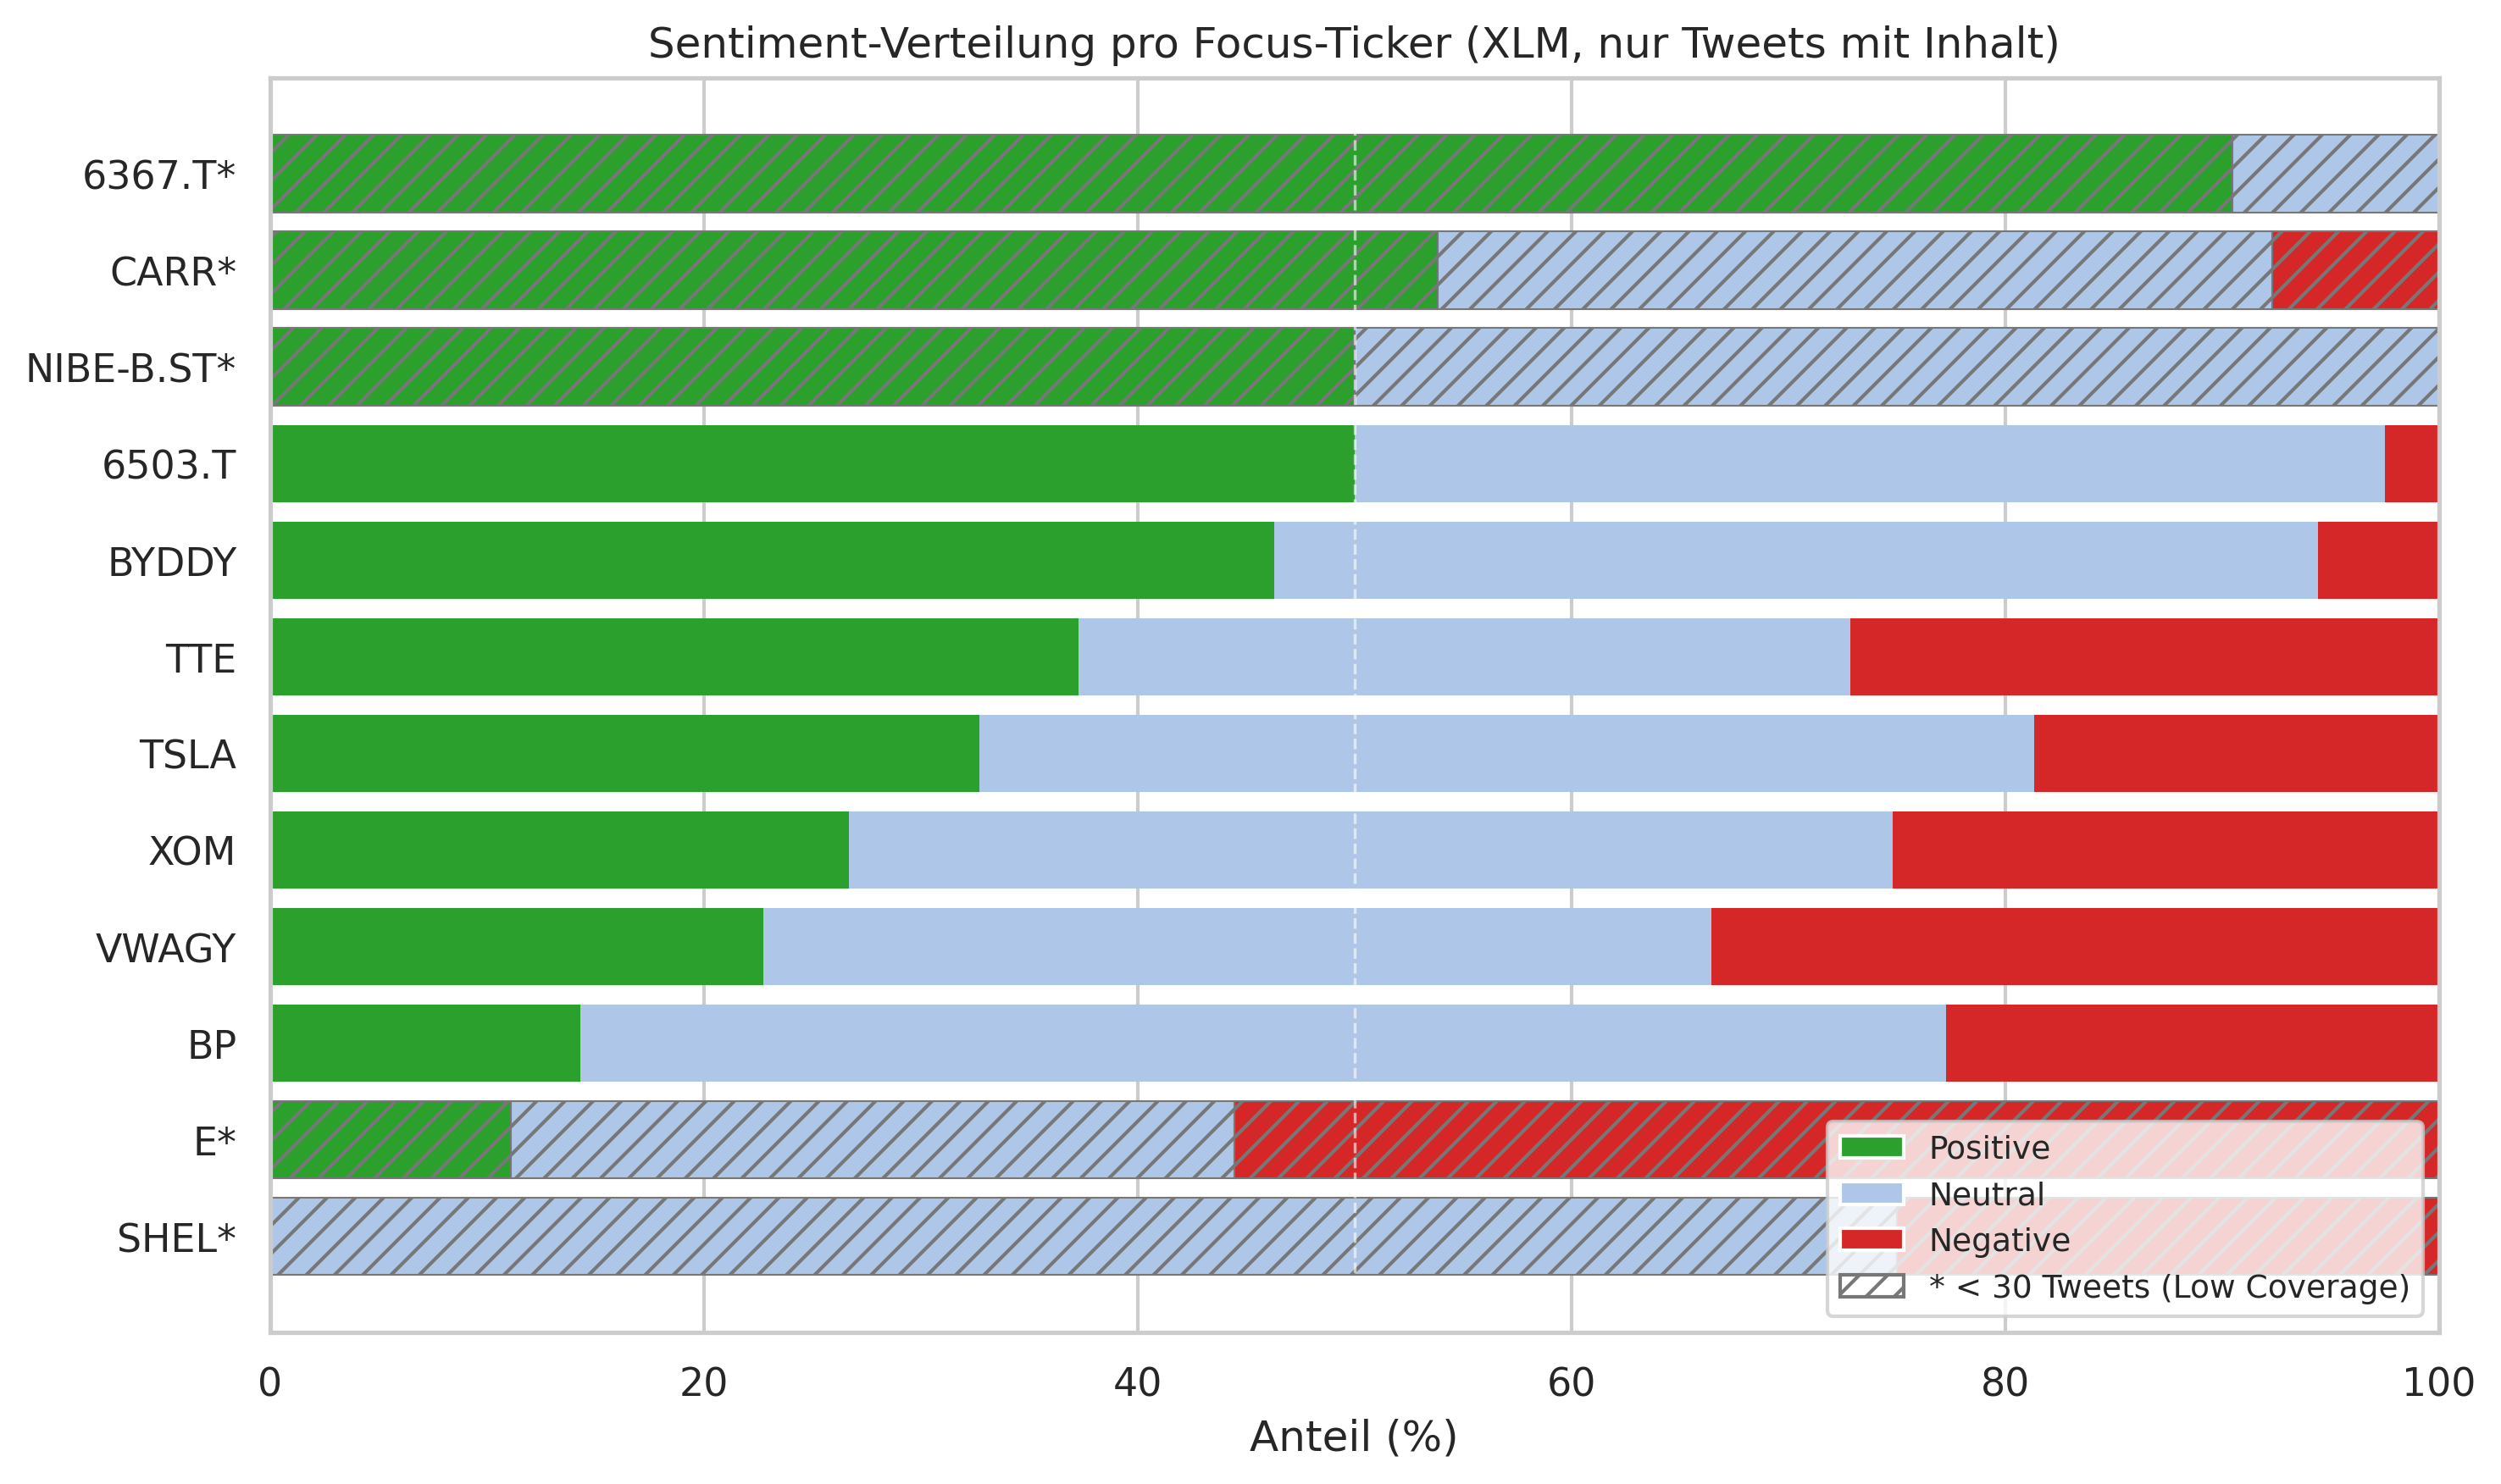
\includegraphics[width=0.85\textwidth]{figures/02_sentiment_analysis/02_sentiment_distribution_by_ticker.png}
  \caption{Sentiment-Verteilung pro Fokus-Ticker (XLM-RoBERTa, nur Tweets mit substantiellem Inhalt). Schraffierte Balken markieren Ticker mit weniger als 30 Tweets (niedrige Abdeckung).}
  \label{fig:label_distribution}
\end{figure}

Über alle Fokus-Ticker verteilt zeigte das XLM-RoBERTa-Modell folgende Labelverteilung: rund 31,9\,\% der verwertbaren Tweets wurden als positiv, 48,5\,\% als neutral und 19,6\,\% als negativ klassifiziert. Der mittlere XLM-Compound-Score auf Tagesaggregat-Ebene betrug $\bar{s} = 0.13$ mit einer Standardabweichung von $\sigma = 0.41$, was auf ein insgesamt leicht positives, aber stark streuendes Signal hindeutet.

Die Übereinstimmung zwischen XLM-RoBERTa und VADER über alle Sprachen betrug 56{,}9\,\% und stieg für den englischsprachigen Teilkorpus auf 57{,}0\,\% an (vgl.\ Abb.~\ref{fig:xlm_vader_scatter}). Der geringe Anstieg beim englischen Teilkorpus deutet darauf hin, dass die sprachliche Homogenisierung allein keinen wesentlichen Unterschied macht; grundlegend unterschiedliche Modellarchitekturen und Trainingskorpora bleiben die Hauptursache für Abweichungen.

\begin{figure}[H]
  \centering
  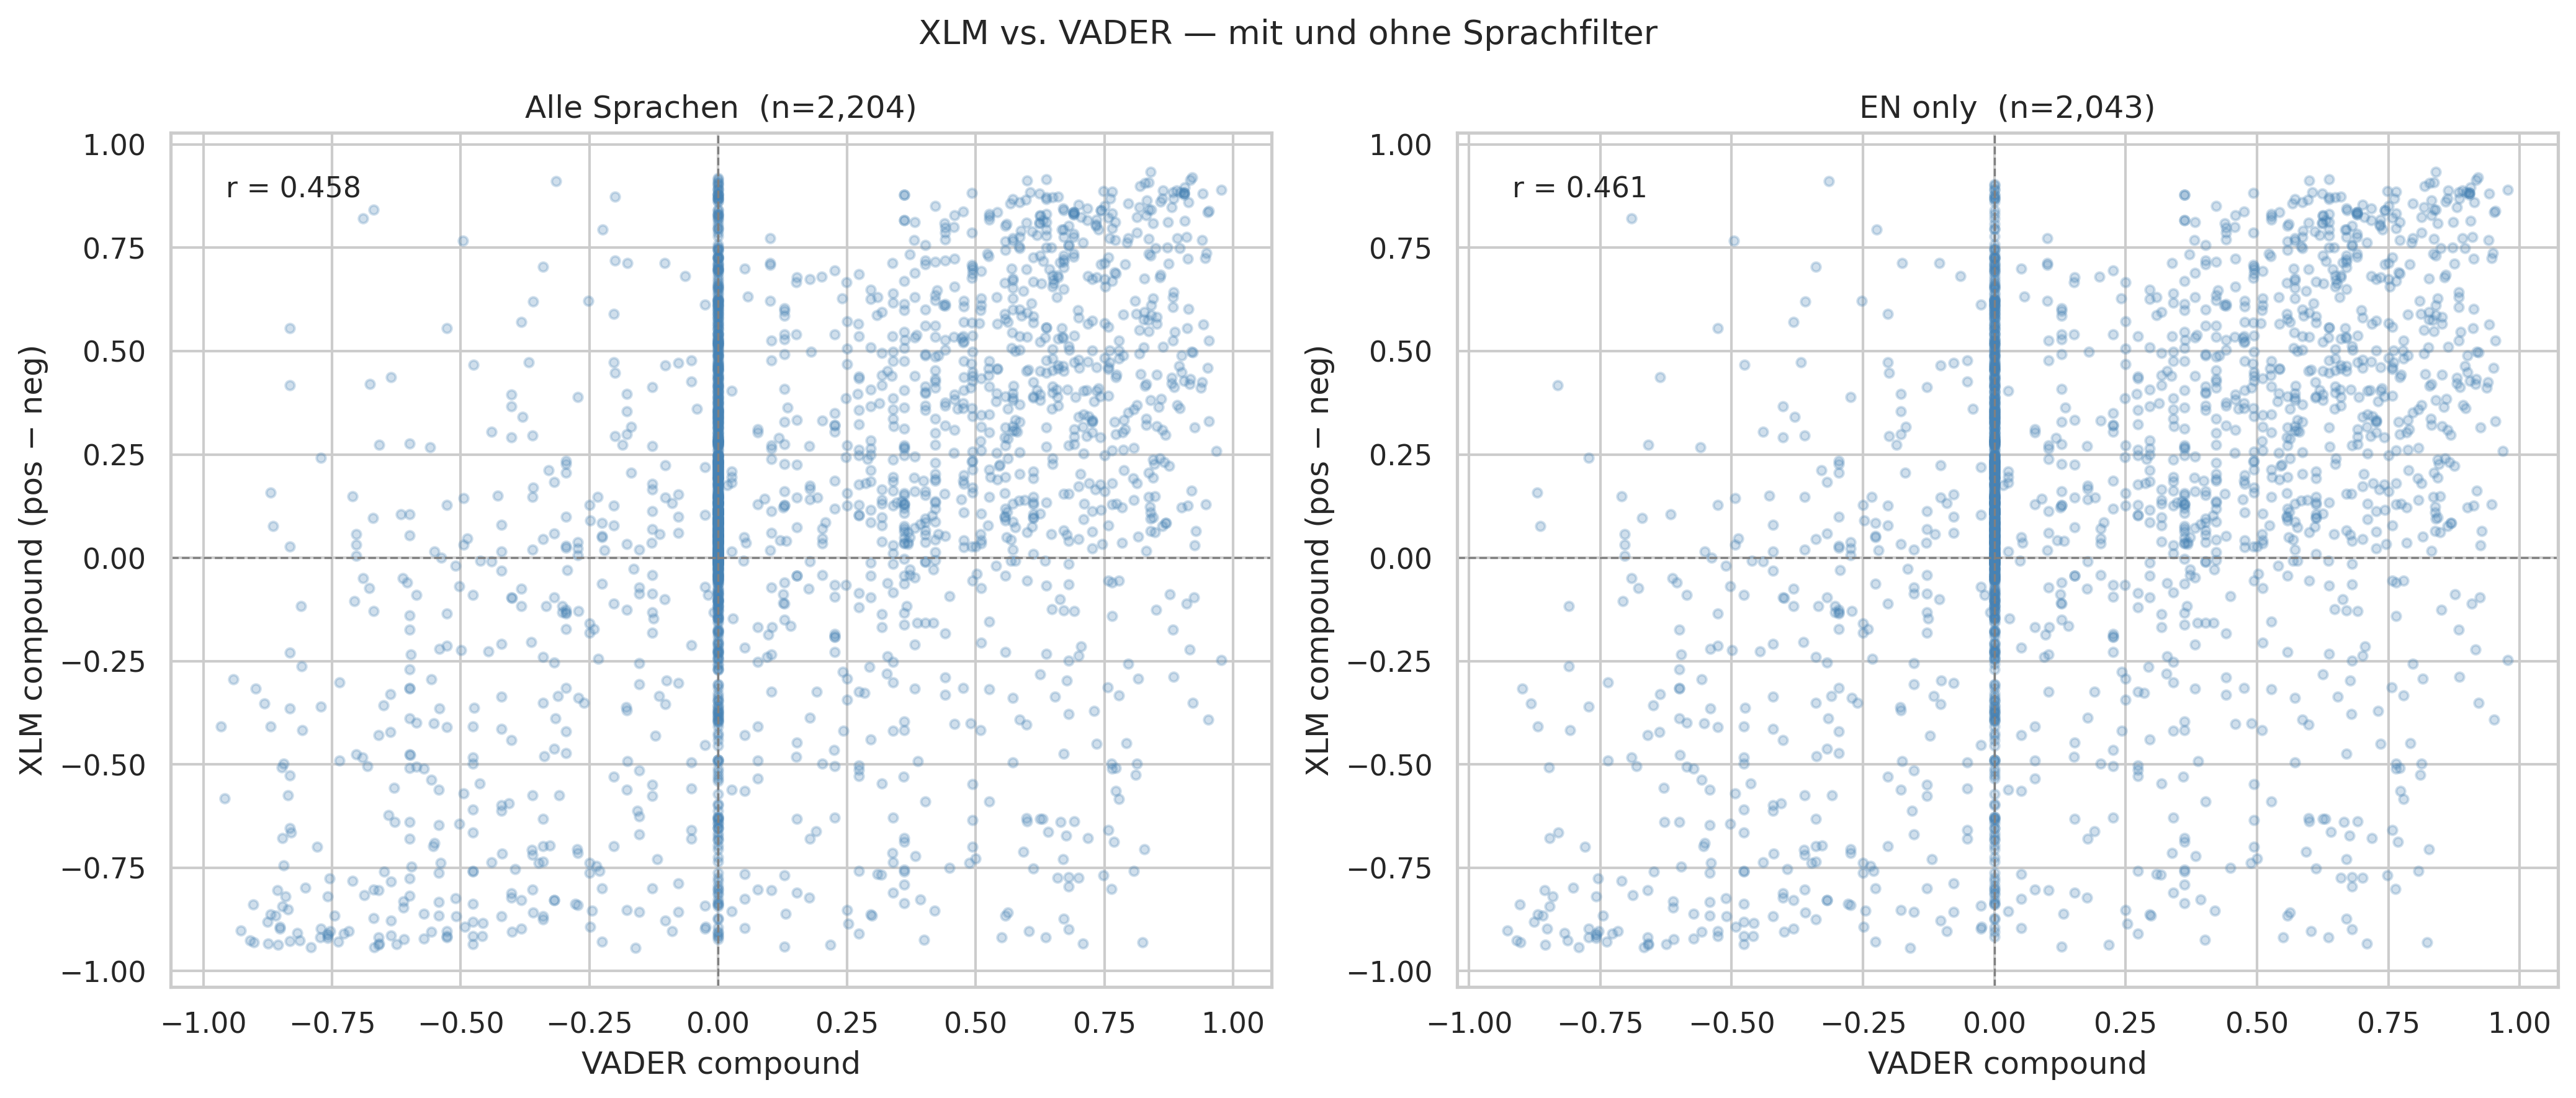
\includegraphics[width=\textwidth]{figures/02_sentiment_analysis/01_xlm_vs_vader_scatter.png}
  \caption{Streudiagramm XLM-RoBERTa- vs.\ VADER-Compound-Score: links alle Sprachen ($n=2\,204$), rechts nur englischsprachige Tweets ($n=2\,043$). Der Pearson-Korrelationskoeffizient $r$ ist jeweils angegeben.}
  \label{fig:xlm_vader_scatter}
\end{figure}

% ─────────────────────────────────────────────────────────────────────────────
\subsection{Lag-Korrelation}
\label{subsec:ergebnisse_lagkorr}

Tabelle~\ref{tab:lag_corr} fasst die stärksten Pearson-Korrelationen je Ticker über alle Lags zusammen.

\begin{table}[H]
\centering
\caption{Stärkste Lag-Korrelationen (Pearson $r$) je Fokus-Ticker mit dem follower-gewichteten Sentiment-Signal. 95\,\%-KI via Fisher-$z$-Transformation. $p_{\mathrm{adj}}$ nach Benjamini-Hochberg-Korrektur.}
\label{tab:lag_corr}
\begin{tabular}{lrrrrrr}
\toprule
\textbf{Ticker} & \textbf{Bester Lag} & \textbf{Pearson $r$} & \textbf{95\,\%-KI} & \textbf{$p_{\mathrm{roh}}$} & \textbf{$p_{\mathrm{adj}}$} & \textbf{$n$} \\
\midrule
E        & Lag 2 & $-0.762$ & $[-0.983,\;+0.367]$ & 0.134 & 0.830 & 5  \\
6367.T   & Lag 1 & $-0.636$ & $[-0.904,\;-0.011]$ & 0.048 & 0.830 & 10 \\
TTE      & Lag 0 & $+0.294$ & $[-0.135,\;+0.630]$ & 0.174 & 0.830 & 23 \\
6503.T   & Lag 0 & $-0.283$ & $[-0.672,\;+0.229]$ & 0.272 & 0.830 & 17 \\
BYDDY    & Lag 3 & $-0.237$ & $[-0.546,\;+0.128]$ & 0.198 & 0.830 & 31 \\
TSLA     & Lag 0 & $-0.234$ & $[-0.447,\;+0.005]$ & 0.055 & 0.830 & 68 \\
XOM      & Lag 3 & $-0.232$ & $[-0.513,\;+0.095]$ & 0.162 & 0.830 & 38 \\
VWAGY    & Lag 3 & $+0.220$ & $[-0.062,\;+0.469]$ & 0.125 & 0.830 & 50 \\
BP       & Lag 0 & $-0.212$ & $[-0.548,\;+0.183]$ & 0.289 & 0.830 & 27 \\
SHEL     & Lag 0 & $+0.196$ & $[-0.830,\;+0.919]$ & 0.752 & 0.952 &  5 \\
\bottomrule
\multicolumn{7}{l}{\footnotesize Kein $p_{\mathrm{adj}} < 0{,}05$ nach BH-FDR-Korrektur (40 Tests gesamt)}
\end{tabular}
\end{table}

Kein Koeffizient blieb nach Anwendung der Benjamini-Hochberg-Korrektur für multiples Testen signifikant ($p_{\mathrm{adj}} < 0{,}05$). Ohne Korrektur wies lediglich 6367.T\,(Daikin) auf Lag~1 einen rohen $p$-Wert unter 0,05 auf ($r = -0.636$, $p_{\mathrm{roh}} = 0.048$, $p_{\mathrm{adj}} = 0.830$). Das breite 95\,\%-Konfidenzintervall dieses Koeffizienten von $[-0.904, -0.011]$ bei $n = 10$ Beobachtungen verdeutlicht die erhebliche Schätzunsicherheit. Dieser Befund ist als zufälliger Treffer bei 40 simultanen Tests zu bewerten und daher nicht inhaltlich interpretierbar.

\begin{figure}[H]
  \centering
  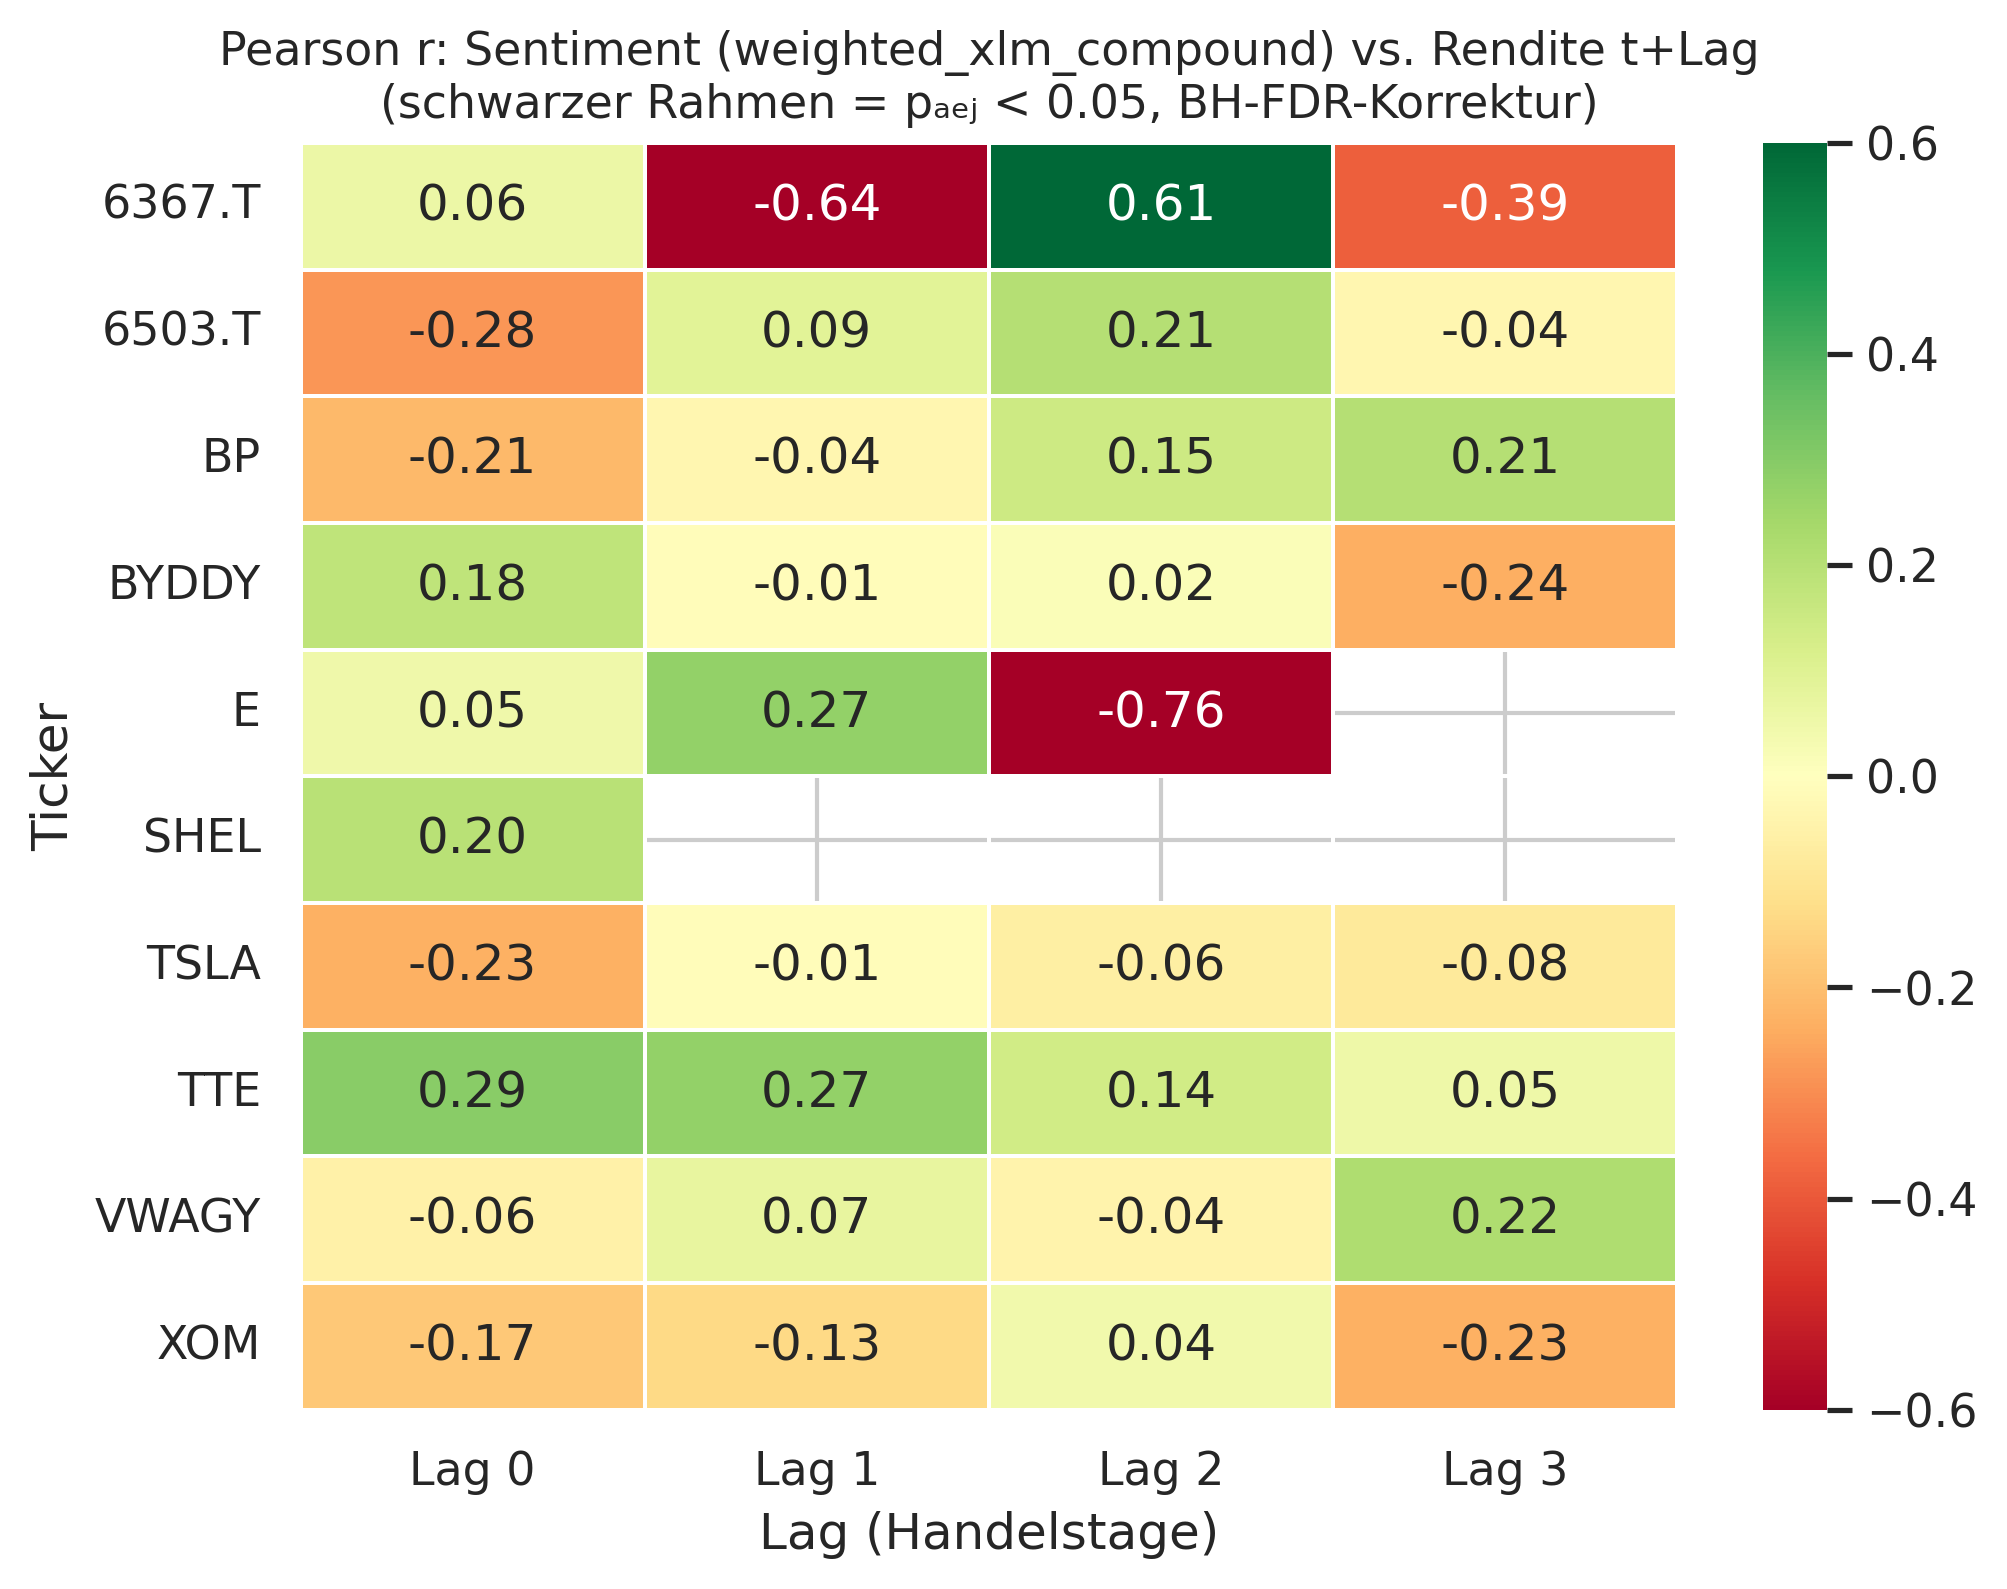
\includegraphics[width=0.72\textwidth]{figures/03_correlation_modeling/01_pearson_heatmap_lags.png}
  \caption{Pearson-Korrelationskoeffizient $r$ zwischen follower-gewichtetem Sentiment am Tag $t$ und Rendite am Tag $t+\text{Lag}$. Da nach BH-FDR-Korrektur kein $p_{\mathrm{adj}} < 0{,}05$ vorliegt, zeigt die Heatmap keine schwarz umrahmten Zellen.}
  \label{fig:pearson_heatmap}
\end{figure}

% ─────────────────────────────────────────────────────────────────────────────
\subsection{Rolling-Korrelation}
\label{subsec:ergebnisse_rolling}

\begin{figure}[H]
  \centering
  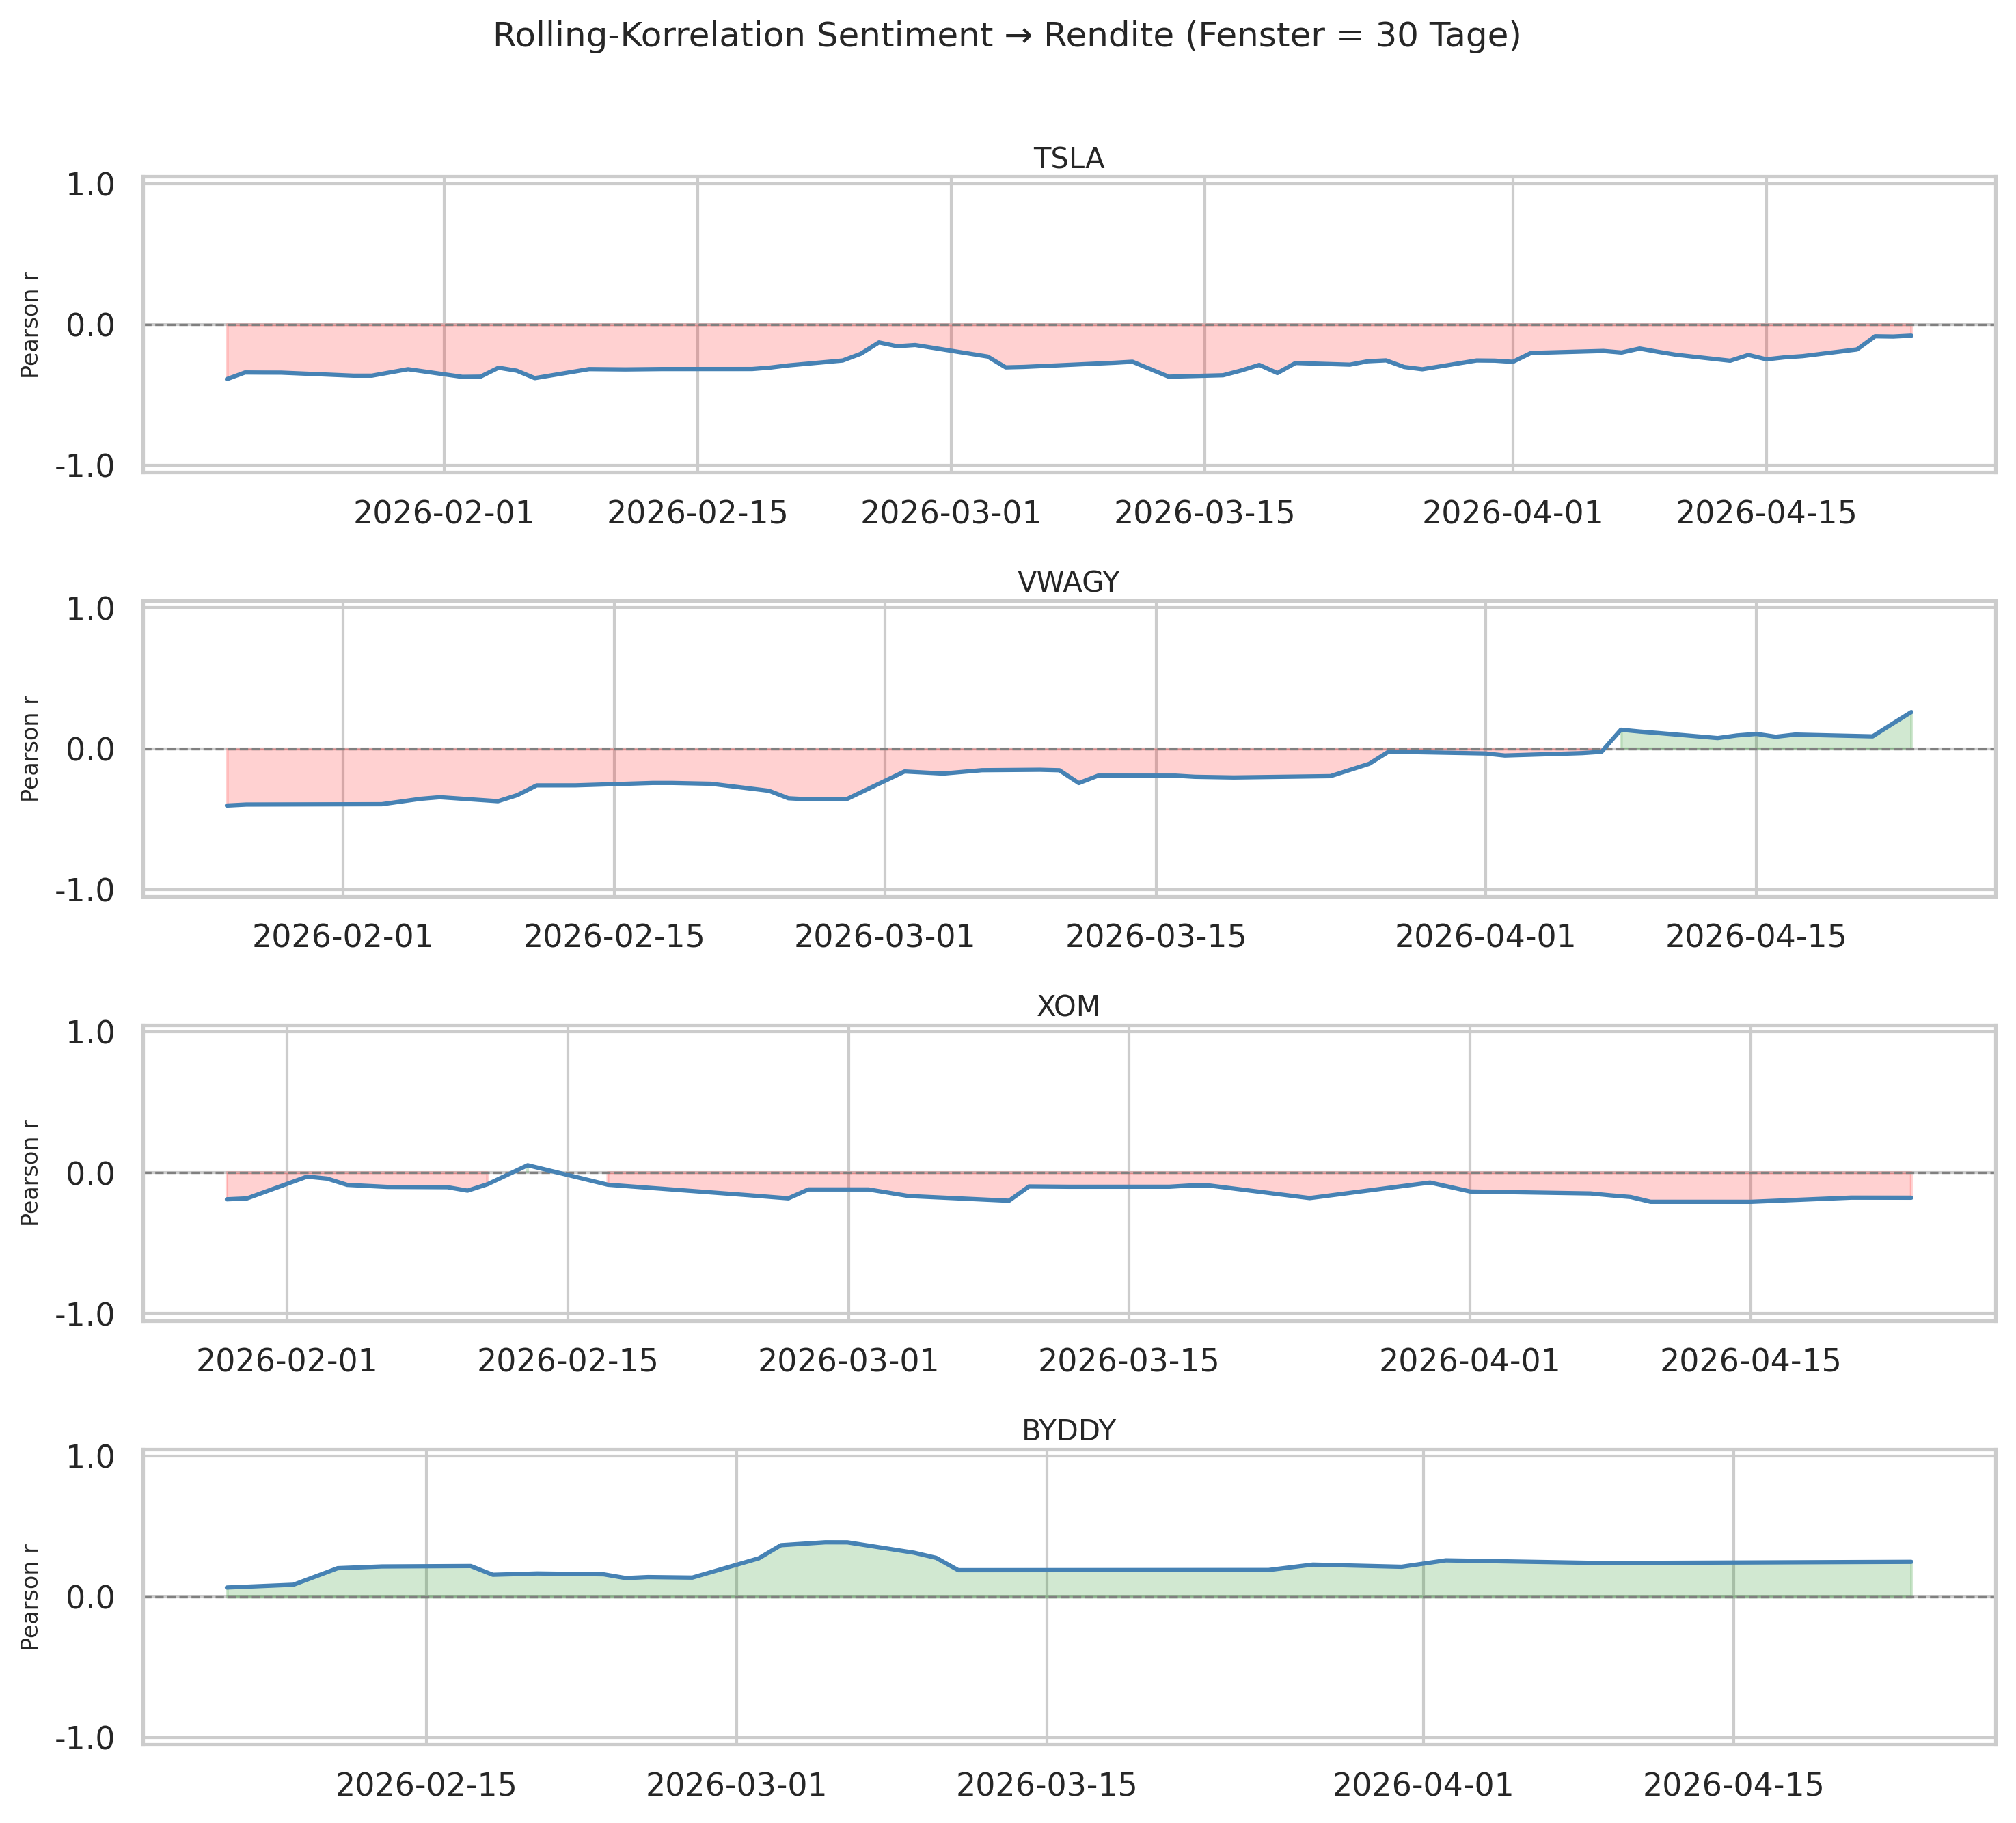
\includegraphics[width=0.9\textwidth]{figures/03_correlation_modeling/02_rolling_correlation.png}
  \caption{Rolling-Korrelation Sentiment $\rightarrow$ Rendite (gleitendes Fenster: 30 Handelstage, Minimum: 10 Punkte) für TSLA, VWAGY, XOM und BYDDY. Grüne Flächen zeigen positive, rote Flächen negative Korrelationsphasen.}
  \label{fig:rolling}
\end{figure}

Die Rolling-Korrelation konnte für vier Ticker berechnet werden: TSLA, VWAGY, XOM und BYDDY. Für alle vier Ticker wechselte das Vorzeichen der Korrelation mehrfach über den Beobachtungszeitraum. Stabile Phasen mit durchgehend positivem oder negativem Zusammenhang waren nicht erkennbar. Dies deutet darauf hin, dass selbst punktuell beobachtbare Zusammenhänge zeitlich nicht robust sind.

% ─────────────────────────────────────────────────────────────────────────────
\subsection{Granger-Kausalitätstest}
\label{subsec:ergebnisse_granger}

Für die vier Ticker mit mindestens 30 Beobachtungen (TSLA, VWAGY, XOM, BYDDY) wurden Granger-Kausalitätstests in beiden Richtungen für Lags 1 bis 3 durchgeführt. Keiner der berechneten F-Test-$p$-Werte unterschritt die Signifikanzschwelle von 0.05. Tabelle~\ref{tab:granger} zeigt die $p$-Werte für die Richtung Sentiment $\rightarrow$ Rendite.

\begin{table}[H]
\centering
\caption{Granger-Kausalitätstest: $p$-Werte (Sentiment $\rightarrow$ Rendite, F-Test)}
\label{tab:granger}
\begin{tabular}{lrrr}
\toprule
\textbf{Ticker} & \textbf{Lag 1} & \textbf{Lag 2} & \textbf{Lag 3} \\
\midrule
TSLA  & 0.957 & 0.658 & 0.602 \\
VWAGY & 0.656 & 0.842 & 0.444 \\
XOM   & 0.544 & 0.712 & 0.349 \\
BYDDY & 0.901 & 0.918 & 0.757 \\
\bottomrule
\end{tabular}
\end{table}

Die $p$-Werte lagen durchgängig deutlich über 0.30, teilweise über 0.90. Es konnte kein Hinweis gefunden werden, dass vergangenes Sentiment die Rendite besser vorhersagt als die Rendite allein.

\begin{figure}[H]
  \centering
  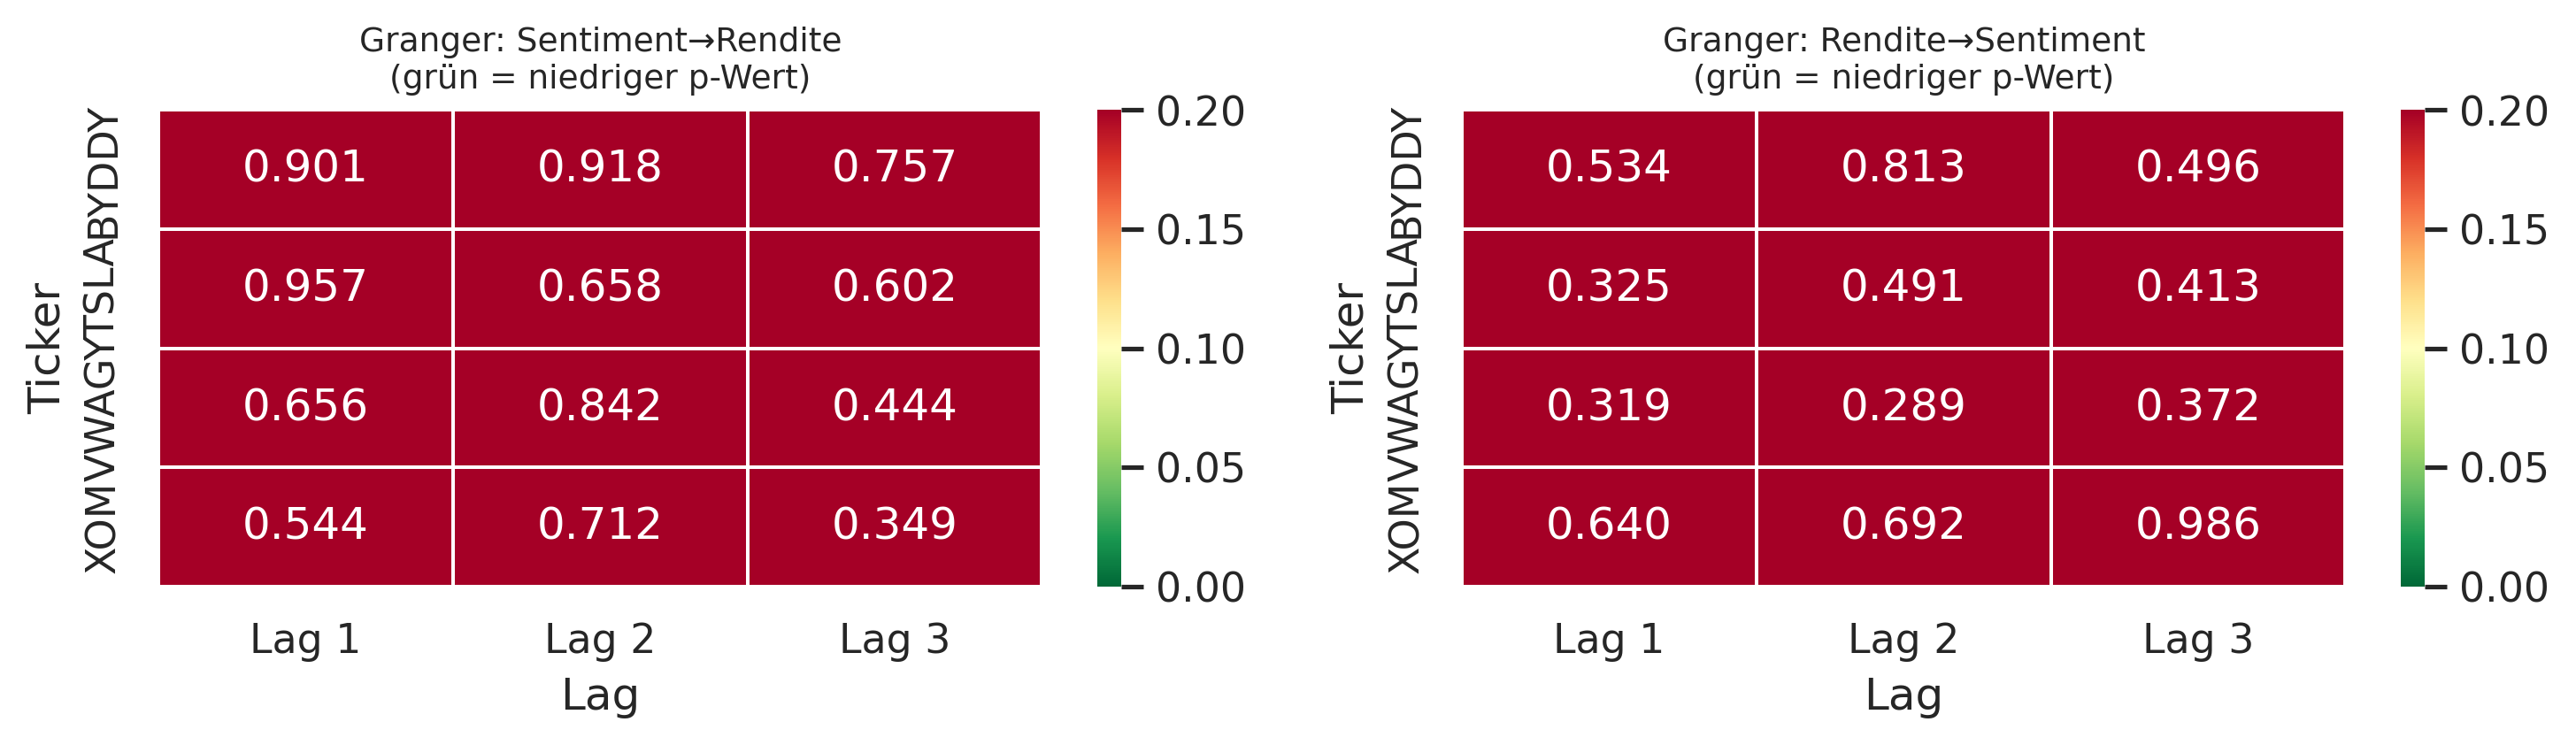
\includegraphics[width=0.85\textwidth]{figures/03_correlation_modeling/03_granger_heatmaps.png}
  \caption{Granger-Kausalitätstest $p$-Werte (F-Test) für beide Richtungen: Sentiment $\rightarrow$ Rendite (links) und Rendite $\rightarrow$ Sentiment (rechts). Grüne Farbe entspricht niedrigen $p$-Werten; kein Wert unterschreitet $p = 0.05$.}
  \label{fig:granger_heatmap}
\end{figure}

% ─────────────────────────────────────────────────────────────────────────────
\subsection{Event-Study}
\label{subsec:ergebnisse_event}

Die Event-Study identifizierte für sechs Ticker ausreichend Ereignisse (mindestens 5 je Richtung). Tabelle~\ref{tab:events} zeigt die Anzahl der positiven und negativen Ereignisse je Ticker.

\begin{table}[H]
\centering
\caption{Event-Study: Anzahl der Ereignisse je Ticker und Richtung}
\label{tab:events}
\begin{tabular}{lrr}
\toprule
\textbf{Ticker} & \textbf{Positive Ereignisse} & \textbf{Negative Ereignisse} \\
\midrule
TSLA  & 11 &  9 \\
VWAGY &  5 &  9 \\
XOM   &  8 &  8 \\
BYDDY &  6 &  5 \\
BP    &  0 &  5 \\
TTE   &  5 &  0 \\
\bottomrule
\end{tabular}
\end{table}

\begin{figure}[H]
  \centering
  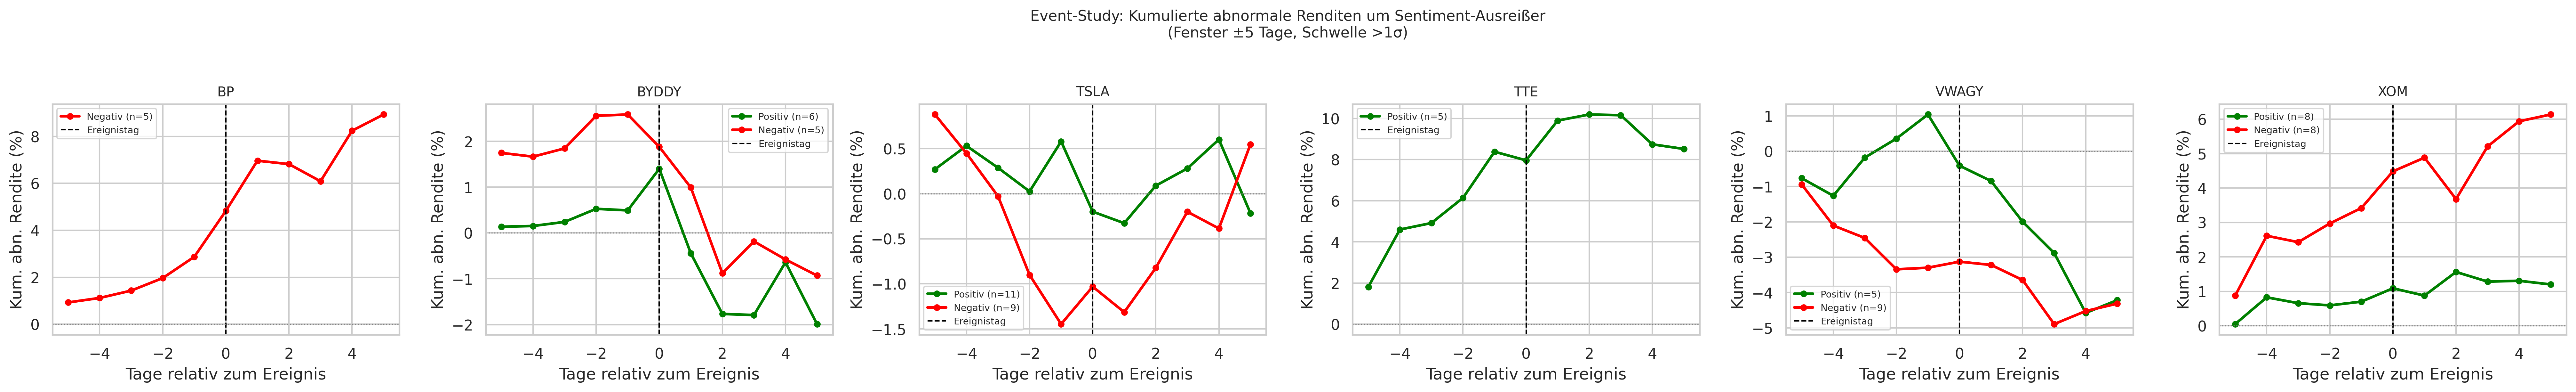
\includegraphics[width=\textwidth]{figures/03_correlation_modeling/04_event_study_car.png}
  \caption{Kumulierte abnormale Renditen (CAR) um Sentiment-Ausrei\ss ertage ($>\!1\sigma$), Fenster $\pm$5 Handelstage, Benchmark: S\&P\,500-Index (\textasciicircum GSPC). Grüne Linien = positive Ereignisse, rote Linien = negative Ereignisse.}
  \label{fig:event_study}
\end{figure}

Die CAR-Profile zeigten keine einheitliche Richtung. Für einzelne Ticker (z.\,B.\ TSLA) war ein gewisses Muster rund um den Ereignistag erkennbar, jedoch ohne statistisch signifikante oder unternehmenübergreifend konsistente Struktur. Positive Sentiment-Ereignisse führten nicht regelmäßig zu positiven abnormalen Renditen -- und umgekehrt.

\newpage

\section{Diskussion}
\label{sec:diskussion}

\subsection{Interpretation der Ergebnisse}

Die Ergebnisse dieser Arbeit liefern keinen robusten, allgemeingültigen Beleg dafür, dass Sentiment-Signale auf X\,(Twitter) Aktienkursrenditen im Beobachtungszeitraum systematisch vorausgingen oder statistisch zuverlässig mit ihnen zusammenhingen. Ohne Korrektur für multiples Testen wies lediglich 6367.T\,(Daikin) auf Lag~1 einen $p$-Wert unter 0,05 auf ($r = -0.636$, $p_{\mathrm{roh}} = 0.048$). Nach Anwendung der Benjamini-Hochberg-FDR-Korrektur \autocite{benjamini1995controlling} über alle 40 simultan durchgeführten Tests stieg dieser Wert auf $p_{\mathrm{adj}} = 0.830$; der Befund ist damit als zufälliger Treffer einzuschätzen. Das 95\,\%-Konfidenzintervall $[-0.904, -0.011]$ bei $n = 10$ verdeutlicht die erhebliche Schätzunsicherheit zusätzlich.

Für die Ticker mit größerer Abdeckung (TSLA, VWAGY, XOM, BYDDY) zeigten sich durchgängig schwache und statistisch nicht signifikante Korrelationskoeffizienten. Auch die Rolling-Korrelation lieferte keine konsistenten Phasen mit robustem Zusammenhang. Der Granger-Test blieb für alle getesteten Ticker ohne signifikantes Ergebnis. Die Event-Study zeigte zwar für einzelne Unternehmen erkennbare CAR-Muster rund um extreme Sentiment-Tage, ein unternehmensübergreifend interpretierbares Signal war jedoch nicht vorhanden.

\subsection{Limitationen}

\paragraph{Multiples Testen.}
Die Lag-Korrelationsanalyse umfasst bis zu 40 simultane Tests (10 Ticker $\times$ 4 Lags). Ohne Korrektur besteht eine hohe Wahrscheinlichkeit für zufällige Signifikanzbefunde. Nach Anwendung der Benjamini-Hochberg-Methode \autocite{benjamini1995controlling} verbleibt kein Test unter der Signifikanzschwelle -- ein Befund, der die Null-Hypothese bestätigt und nicht schwächt.

\paragraph{Stationarität.}
Der Granger-Test setzt Stationarität der Eingangszeitreihen voraus. Für alle vier Ticker, die den Granger-Test durchliefen, wurden beide Reihen (Sentiment-Signal und tägliche Renditen) vorab mit dem ADF-Test geprüft \autocite{dickey1979distribution}. Sämtliche Reihen wiesen $p < 0{,}001$ auf -- die Stationaritätsvoraussetzung war erfüllt.

\paragraph{Beobachtungszeitraum.}
Die zentrale Einschränkung dieser Arbeit ist die kurze Überlappungszeit zwischen den verfügbaren Sentiment-Daten und den Tagespreisen. Der nutzbare Zeitraum umfasste nur etwa vier Monate (Januar bis April 2026). Dies führt zu geringen Stichprobengrößen, insbesondere für Ticker mit seltenerer Tweet-Aktivität. Viele statistische Methoden -- insbesondere Granger-Tests und Rolling-Korrelationen -- setzten Mindestbeobachtungszahlen voraus, die nur für eine Teilmenge der Fokus-Ticker erfüllt waren. Die statistische Power der gesamten Analyse ist damit grundsätzlich begrenzt.

\paragraph{Ungleiche Abdeckung.}
Die Tweet-Aktivität war stark auf einzelne Ticker konzentriert. TSLA vereinte allein fast die Hälfte aller Sentiment-Tage. Unternehmen wie NIBE\,(NIBE-B.ST) oder Carrier\,(CARR) hatten im Untersuchungszeitraum kaum Erwähnung auf X\,(Twitter), sodass für diese Ticker keine aussagekräftigen Analysen möglich waren.

\paragraph{Crawler-Einschränkungen.}
Die Datenerhebung über X\,(Twitter) unterliegt technischen und rechtlichen Einschränkungen. Es ist anzunehmen, dass nicht alle relevanten Tweets erfasst wurden. Insbesondere Beiträge mit geringer Sichtbarkeit oder von kleineren Accounts könnten systematisch unterrepräsentiert sein.

\paragraph{Aggregationsebene.}
Die Analyse auf Tagesbasis kann intraday auftretende Zusammenhänge zwischen Sentiment und Kursreaktion nicht erfassen. Gerade bei News-getriebenen Kursausschlägen wäre eine höhere zeitliche Auflösung wünschenswert.

\paragraph{Kausalität und Konfundierung.}
Selbst bei signifikanten Korrelationen oder positiven Granger-Tests wäre keine kausale Interpretation zulässig. Sowohl Sentiment als auch Renditen können gemeinsam von externen Faktoren (z.\,B.\ Konjunkturdaten, geopolitische Ereignisse, Analystenmeinungen) getrieben werden, ohne dass ein direkter Wirkungspfad zwischen ihnen besteht.

\subsection{Einordnung in den Forschungskontext}

Die vorliegende Arbeit reiht sich in ein breites Forschungsfeld ein, das sich mit der Vorhersagbarkeit von Aktienrenditen durch Social-Media-Daten befasst. Frühe Studien, darunter \textcite{bollen2011twitter}, berichteten von positiven Ergebnissen bei der Nutzung von Twitter-Sentiment zur Vorhersage des Dow-Jones-Index. Spätere Replikationsstudien zeigten jedoch, dass solche Zusammenhänge häufig instabil, zeitraumabhängig und schwer generalisierbar sind \autocite{ranco2015effects}. Die vorliegende Arbeit bestätigt diesen vorsichtigen Befund: Ein generelles prädiktives Signal aus Social-Media-Sentiment ist im kurzen Untersuchungszeitraum nicht nachweisbar.

\newpage

\section{Fazit}
\label{sec:fazit}

Die vorliegende Arbeit untersuchte, ob aus dem täglichen Sentiment auf X\,(Twitter) ein statistisch signifikanter Zusammenhang mit den Tagesrenditen von zwölf Fokus-Unternehmen aus den Bereichen Energie, Wärmepumpen und Elektromobilität abzuleiten ist. Dafür wurden ein selbst erhobener Tweet-Datensatz und historische Börsenkursdaten mithilfe eines multilingualen Transformer-Modells, eines lexikonbasierten Baseline-Verfahrens sowie vier statistischer Analysemethoden ausgewertet.

Die zentralen Befunde lassen sich wie folgt zusammenfassen: Im beobachteten Zeitraum von rund vier Monaten (Januar bis April 2026) fand sich kein konsistentes Muster, das auf eine systematische Vorhersagbarkeit von Kursrenditen durch Twitter-Sentiment hinweist. Nach Anwendung der Benjamini-Hochberg-FDR-Korrektur für multiples Testen verblieb keine Pearson-Korrelation unter der Signifikanzschwelle von $\alpha = 0{,}05$ -- der einzige rohe Befund (Daikin, Lag~1, $p_{\mathrm{roh}} = 0{,}048$) wies nach Korrektur $p_{\mathrm{adj}} = 0{,}830$ auf und ist als zufälliger Treffer bei 40 simultanen Tests einzuordnen. Granger-Tests blieben für alle Ticker ohne signifikantes Ergebnis. Rolling-Korrelationen zeigten keine stabilen Zusammenhangsphasen. Event-Study-Profile variierten stark zwischen Unternehmen und Richtungen, ohne ein unternehmensübergreifendes Signal zu erzeugen.

Diese Ergebnisse sind in erster Linie durch den kurzen Beobachtungszeitraum und die damit verbundene geringe statistische Power zu erklären. Eine Replikation mit einem längeren Datensatz -- idealerweise über mehrere Jahre und über verschiedene Marktphasen -- wäre notwendig, um belastbarere Aussagen treffen zu können. Darüber hinaus könnte eine höhere zeitliche Auflösung (intraday), eine feingranularere Segmentierung nach Account-Typen sowie eine gezieltere Vorverarbeitung von mehrsprachigen Inhalten die Aussagekraft zukünftiger Analysen verbessern.

Methodisch leistet die Arbeit einen Beitrag, indem sie ein reproduzierbares, modulares Analyse-Pipeline-Design zeigt, das Datenerhebung, Sentiment-Quantifizierung und statistische Modellierung transparent trennt und für jeden Analyseschritt Qualitäts- und Coverage-Prüfungen dokumentiert. Die Implementierung der Retweet-Separation, der Bot-Filterung sowie des Overlap-Reports sind Bestandteile, die sich in ähnlichen Projekten wiederverwenden lassen.

\newpage

% ── Bibliography ─────────────────────────────────────────────────────────────
\printbibliography[heading=bibintoc, title={Literaturverzeichnis}]

\end{document}
